\documentclass[conference]{IEEEtran}
\usepackage{cite}
\usepackage{amsmath,amssymb}
\usepackage{graphicx}
\usepackage{booktabs,tabularx,array}
\usepackage{xcolor}
\usepackage{tikz}
\definecolor{cuaBlue}{HTML}{2F6DAA}
\definecolor{cuaOrange}{HTML}{E0832B}
\definecolor{cuaGreen}{HTML}{1B5E4B}
\definecolor{cuaPurple}{HTML}{8068A8}
\definecolor{cuaTeal}{HTML}{3A9AA0}
\definecolor{cuaGold}{HTML}{D6A52F}
\definecolor{cuaPos}{HTML}{2E8B57}
\definecolor{cuaNeg}{HTML}{C4473D}
\definecolor{cuaGrey}{HTML}{E3E7EA}
\definecolor{cuaText}{HTML}{6B7075}
\definecolor{cuaArrow}{HTML}{6B7075}
\usetikzlibrary{matrix,arrows.meta,positioning,fit,calc,backgrounds}
\usepackage[hidelinks]{hyperref}
\urlstyle{same}
\newcolumntype{Y}{>{\raggedright\arraybackslash}X}

\newcommand{\todo}[1]{\textcolor{red}{\textbf{[#1]}}}

\begin{document}

\title{Class-Aware Augmentation Selection for Multi-Class Object Detection}
\maketitle

% \begin{abstract}
% Written last (Stage 7).
% \end{abstract}

\begin{IEEEkeywords}
augmentation policy, data augmentation, gradient alignment, infrastructure inspection, multi-class images, object detection
\end{IEEEkeywords}

\section{Introduction}
\label{sec:intro}

Object detection underlies applications ranging from everyday scene understanding to the automated inspection of roads and bridges~\cite{everingham2010voc,shang2024automated,zheng2024deep,vision2025inspection}, and in most of them a detector must locate and classify objects of several classes within the same image. Achieving reliable detection remains challenging, because the appearance of each class varies with illumination, viewpoint, background and image quality, and a training set rarely covers this variation in full. The difficulty is compounded by differences among the classes themselves. Some are identified mainly by shape or fine structure, such as thin cracks in pavement and concrete~\cite{arya2024rdd,flotzinger2024dacl10k}, whereas others are identified mainly by colour or texture, such as rust on steel~\cite{flotzinger2024dacl10k}, and everyday scenes routinely place small, thin objects beside large, compact ones~\cite{everingham2010voc}. Consequently, improving detection requires exposing the detector to a wider range of visual conditions while preserving the cues that distinguish each class.

Data augmentation addresses the first part of this requirement by applying controlled edits, such as geometric, colour and image-quality transformations, to training images, so that the detector learns from more varied conditions without additional annotation. The effectiveness of an edit, however, depends on whether it preserves the cues that define each class. An edit that alters the cue a class depends on, such as colour for rust and efflorescence or fine texture for hairline cracks, may therefore affect that class differently from classes that rely on other cues, such as overall shape. The same edit may provide useful variation for one class while removing information that another class needs. In detection, this tension arises within a single training image rather than only between images: standard pipelines edit the whole image, so every object in it receives the same edit, and an edit that helps the detector learn one class may hinder another class in the same image. Such conflicts are easily overlooked, because augmentation is usually judged by accuracy averaged over classes, and gains in average accuracy can coexist with losses for individual classes~\cite{kirichenko2023}. This motivates augmentation that accounts for how each class responds to each edit, and that chooses the edit for an image according to the classes the image contains.

Existing augmentation methods have progressively moved toward this goal, but each stops short of it. AutoAugment and RandAugment search for or simplify one policy shared by the whole dataset~\cite{cubuk2019auto,cubuk2020rand}, and detection-specific extensions add edits restricted to annotated boxes or adapt the policy to object scale~\cite{zoph2020det,chen2021scale}; none of these policies, however, depends on the class of the objects being edited. Class-aware approaches recognize that classes may require different augmentations~\cite{tsuchiya2019,yoo2023,cheung2022adaaug}, in some cases by setting augmentation probabilities per class before training~\cite{rdd_detectron2}. Because these policies are fixed before or apart from detector training, they cannot follow changes in what each class needs as learning progresses. Online methods remove this restriction by adapting augmentation from the feedback of the evolving model, but the feedback they use introduces two further limitations. Tolerance-based controllers such as CTAugment and CUDA adjust augmentation according to whether the model still recognizes augmented examples~\cite{berthelot2020,ahn2023cuda}, which indicates what the model can already handle rather than whether training on the edit improves it. Benefit-based methods such as BDA, DDAS and MADAug measure that improvement through a held-out loss~\cite{lu2023bda,liu2021ddas,hou2023madaug}, but they compute it over all classes together, so an edit that helps frequent classes can be preferred even when it harms a rare one. Moreover, the class-aware methods among them are formulated for classification, where each training sample carries one label, and therefore do not specify which class should govern an image that contains several.

This gap matters in detection because the classes in one image may disagree about an edit. If an edit helps the detector learn one class in an image but hinders another, a policy guided by pooled feedback sees only the net effect and applies the same preference to every image, whereas a policy keyed to a single class must ignore the other. What is needed instead is a measure of how much each edit helps each class learn, combined into one decision for the image that respects every class it contains.

To meet this need, we propose Class-Utility Augmentation (CUA), an online augmentation policy that selects the edit for each training image from the classes present in it. CUA is built around the \emph{class utility} of an edit, defined as the estimated amount that the edit helps a given class learn. CUA estimates this utility during training with a first-order argument from training-influence analysis~\cite{pruthi2020tracin}: if a gradient step on the edited image would reduce a class's loss on a held-out \emph{reference set} more than a step on the original image would, the edit currently benefits that class. For each training image, CUA then averages the utilities of the classes present, removes any edit that is reliably harmful to one of them, and samples a single edit from the remainder, with ``no edit'' always available as a candidate of zero utility (Fig.~\ref{fig:teaser}). Because the utilities are re-estimated from the current detector, the preferred edits can change as training proceeds, and because CUA requires no policy network and no separate search phase, it adds only a periodic gradient computation to standard training.

The value of CUA rests on the premise that classes respond differently to the same edit, so we examine this premise before evaluating the method. Across road damage (RDD2022), bridge damage (dacl10k) and everyday objects (PASCAL VOC)~\cite{everingham2010voc}, and with two detector families, Faster R-CNN~\cite{ren2017faster} and RetinaNet~\cite{lin2017focal}, we train detectors with one edit at a time to measure its effect on each class. We then compare CUA with shared-utility augmentation, an otherwise identical policy that averages utility over all classes, so that any difference between the two reflects class information alone. \todo{One-sentence summary of findings: which edits affect classes in opposite directions; CUA minus shared-utility on test macro AP50 with 95\% intervals; rank agreement between estimated utilities and measured effects.} In summary, this paper makes the following contributions:

\begin{enumerate}
    \item Class-Utility Augmentation, an online augmentation policy for multi-class object detection that estimates how much each edit helps each class learn and selects one edit per image from the classes it contains, with a no-edit option and a per-class harm block.
    \item A controlled measurement of how individual edits affect each class in detection, across three domains and two detector families.
    \item A comparison with a shared-utility counterpart that differs from CUA only in class information, together with standard augmentation baselines, and a test of whether the estimated class utilities agree with the measured per-class effects.
\end{enumerate}

\begin{figure}[t]
\centering
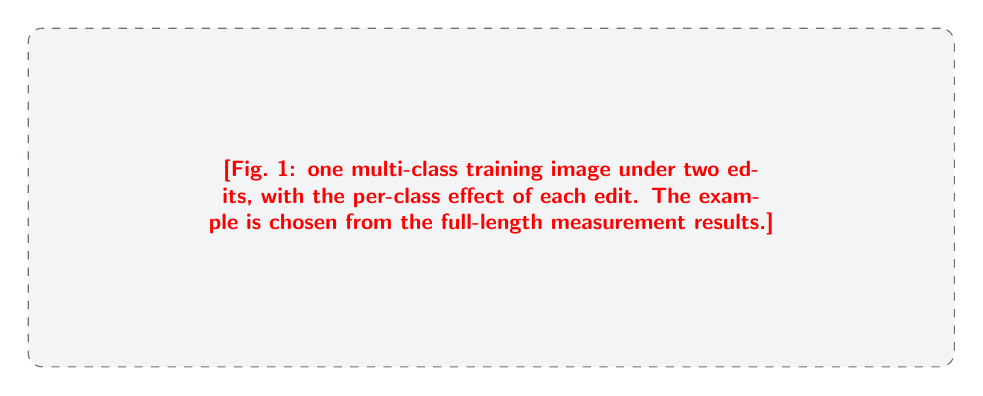
\begin{tikzpicture}
  \node[draw=cuaText, dashed, rounded corners=5pt, fill=cuaGrey!45, minimum width=0.97\columnwidth, minimum height=4.3cm, text width=0.8\columnwidth, align=center, font=\sffamily\footnotesize] {\todo{Fig.~1: one multi-class training image under two edits, with the per-class effect of each edit. The example is chosen from the full-length measurement results.}};
\end{tikzpicture}
\caption[Teaser]{\todo{Caption written once the example is chosen.}}
\label{fig:teaser}
\end{figure}

\section{Related Work}
\label{sec:related}

\noindent\textbf{Augmentation policies for object detection.} Automatic augmentation began by treating the choice of edits as a search over a whole dataset. AutoAugment searches over operations, probabilities and magnitudes with validation accuracy as the reward~\cite{cubuk2019auto}; because this search is expensive, RandAugment reduces it to two shared parameters~\cite{cubuk2020rand}, and TrivialAugment goes further, showing that sampling one edit and strength uniformly at random is a strong baseline that needs no tuning~\cite{muller2021trivial}. Detection raises an additional question, namely where in the image an edit should act. Zoph \emph{et al.} answer it by learning policies that include edits restricted to the content of each box~\cite{zoph2020det}, Scale-Aware AutoAug by conditioning image- and box-level policies on object scale~\cite{chen2021scale}, and InterAug by constructing a tuning-free detection policy~\cite{thopalli2023interaug}. Inspection work has followed the same pattern with recipes designed for damage imagery, such as bounding-box augmentation combined with samples from generative adversarial networks~\cite{aghayan2024} or content- and perspective-aware cut-and-paste of damage~\cite{rdd_cutpaste}. Although these methods differ in how the policy is found, they share one property: the edit for an image is drawn from a single distribution, conditioned at most on location or scale, which implicitly assumes that every class benefits from the same edits.

\noindent\textbf{Class-aware augmentation.} Evidence from recognition suggests that this assumption does not always hold. Kirichenko \emph{et al.} show that augmentation which raises average ImageNet accuracy can lower the accuracy of individual classes~\cite{kirichenko2023}, and Tsuchiya \emph{et al.} find that augmentation methods for road-damage classification differ in their effect on individual damage classes~\cite{tsuchiya2019}. Several methods have therefore made augmentation depend on the class. Yoo and Kang derive class-specific parameters from a classifier trained beforehand~\cite{yoo2023}, AdaAug learns class-adaptive policies in a separate search~\cite{cheung2022adaaug}, CUDA updates a severity for each class during training~\cite{ahn2023cuda}, and Pham \emph{et al.} set augmentation probabilities for each damage type from an exploration of the data~\cite{rdd_detectron2}. These methods share a limitation that becomes decisive in detection. The classification methods select the augmentation by the label of a sample, which has no answer when an image contains objects of several classes, while the detection recipe sidesteps the question by fixing its probabilities before training. PSIS, the closest detection counterpart, adapts to per-class detection accuracy during training, but it controls how many instance-switched samples each class receives rather than which edit each image receives~\cite{wang2019psis}. A method for multi-class detection must therefore choose edits from the whole set of classes in an image, and must do so as the needs of the detector change during training.

\noindent\textbf{Adapting augmentation during training.} Online methods make this second requirement possible by updating augmentation from the model as it trains, but they differ in the feedback they treat as evidence that an edit is useful. Tolerance-based methods ask whether the current model still recognizes, or tolerates, augmented examples. CTAugment adjusts per-operation magnitudes from predictions on augmented labeled data, pooled over classes~\cite{berthelot2020}; CUDA raises or lowers the severity of each class according to how well its augmented examples are recognized~\cite{ahn2023cuda}; and TeachAugment keeps learned transformations recognizable to a teacher while making them hard for the target model~\cite{suzuki2022teach}. Recognition, however, reflects what the model can already handle rather than what it gains from training on the edit, which is the quantity augmentation is meant to increase. Benefit-based methods measure this gain more directly. BDA rewards an augmentation by the training gain it yields over a paired unaugmented reference~\cite{lu2023bda}, DDAS uses a one-step gradient update to estimate how the augmentation distribution affects a held-out loss, including for detection~\cite{liu2021ddas}, MADAug learns an input-dependent policy through a bilevel validation objective~\cite{hou2023madaug}, and RangeAugment and AdaAugment adapt magnitudes from task-loss feedback~\cite{mehta2022rangeaugment,yang2025adaaugment}. Their common limitation is that the benefit is computed over all classes together, so a gain for frequent classes can outweigh a loss for a rare one, which is precisely the trade-off that a multi-class image creates. Estimating the gain separately for each class need not be costly. TracIn measures the influence of a training example on a test loss through the alignment of their gradients~\cite{pruthi2020tracin}, and CUA applies the same first-order argument to edited versus unedited images and to a separate reference loss for each class.

Table~\ref{tab:policies} places these methods on two axes: the signal that guides augmentation, and whether that signal is resolved by class. Each ingredient of CUA has a precedent among them, including class conditioning, online adaptation, benefit signals and gradient-alignment estimates. None of them, however, keeps a benefit estimate separate for each class and combines these estimates into one decision for an image that contains several classes, with leaving the image unedited as an explicit option. CUA is designed for this case, and its comparison with shared-utility augmentation, which removes the class information and nothing else, tests whether the class information matters.

\begin{table*}[t]
\caption{Augmentation Methods Grouped by Feedback Signal and Class Resolution}
\label{tab:policies}
\centering
\small
\setlength{\tabcolsep}{3.5pt}
\renewcommand{\arraystretch}{1.12}
\begin{tabularx}{\textwidth}{@{}p{0.155\textwidth}p{0.145\textwidth}p{0.115\textwidth}p{0.06\textwidth}Y@{}}
\toprule
\textbf{Method} & \textbf{Original setting} & \textbf{Signal} & \textbf{Per class} & \textbf{Relation to CUA} \\
\midrule
TrivialAugment~\cite{muller2021trivial} & Classification & None & No & Uniform augmentation baseline in our comparison. \\
Zoph \emph{et al.}~\cite{zoph2020det} & Detection & Offline search & No & Box-level operations; one policy for the dataset. \\
Scale-Aware AutoAug~\cite{chen2021scale} & Detection & Offline search & No & Conditioned on object scale rather than class. \\
Pham \emph{et al.}~\cite{rdd_detectron2} & Road-damage detection & Data exploration & Yes & Per-class probabilities fixed before training. \\
PSIS~\cite{wang2019psis} & Detection & Validation AP & Yes & Adapts per-class instance switching, not the edit. \\
Yoo and Kang~\cite{yoo2023} & Classification & Offline, then schedule & Yes & One label per sample selects the parameters. \\
AdaAug~\cite{cheung2022adaaug} & Classification & Learned offline & Yes & One label per sample; policy reused after search. \\
CTAugment~\cite{berthelot2020} & Semi-supervised classification & Tolerance & No & Statistics pooled across classes. \\
CUDA~\cite{ahn2023cuda} & Long-tailed classification & Tolerance & Yes & One label per sample selects the severity. \\
BDA~\cite{lu2023bda} & Classification & Benefit & No & Paired training gain, pooled across classes. \\
DDAS~\cite{liu2021ddas} & Classification, detection & Benefit & No & One-step held-out loss, pooled across classes. \\
MADAug~\cite{hou2023madaug} & Classification & Benefit (learned) & Implicit & Input-dependent policy learned from one pooled validation loss. \\
RangeAugment~\cite{mehta2022rangeaugment} & Classification, detection & Task loss (learned) & No & Learns magnitude ranges online. \\
AdaAugment~\cite{yang2025adaaugment} & Classification & Loss feedback (learned) & No & Instance-level magnitudes from an actor--critic controller. \\
\midrule
CUA (ours) & Multi-class detection & Benefit & Yes & Per-class benefit combined over the classes in each image; no-edit option and per-class harm block. \\
\bottomrule
\end{tabularx}
\vspace{3pt}
\begin{minipage}{\textwidth}
\footnotesize
Signal: \emph{tolerance} = whether the current model still recognizes augmented examples; \emph{benefit} = whether training on augmented data reduces a held-out or reference loss. CTAugment is the augmentation component of ReMixMatch.
\end{minipage}
\end{table*}

\section{Class-Utility Augmentation}
\label{sec:method}

CUA decides, for every training image, which single edit to apply on top of a fixed base recipe. It makes this decision by keeping an estimate of how much each edit currently helps each class learn, and by combining these estimates over the classes present in the image. Fig.~\ref{fig:framework} shows the two parts of the method: an estimator that periodically updates a table of class utilities from gradients (Sec.~\ref{sec:method_estimator}), and an image policy that reads this table to choose the edit for each image (Sec.~\ref{sec:method_policy}). We first fix the notation and the augmentation that every image receives regardless of the policy.

\begin{figure*}[t]
\centering
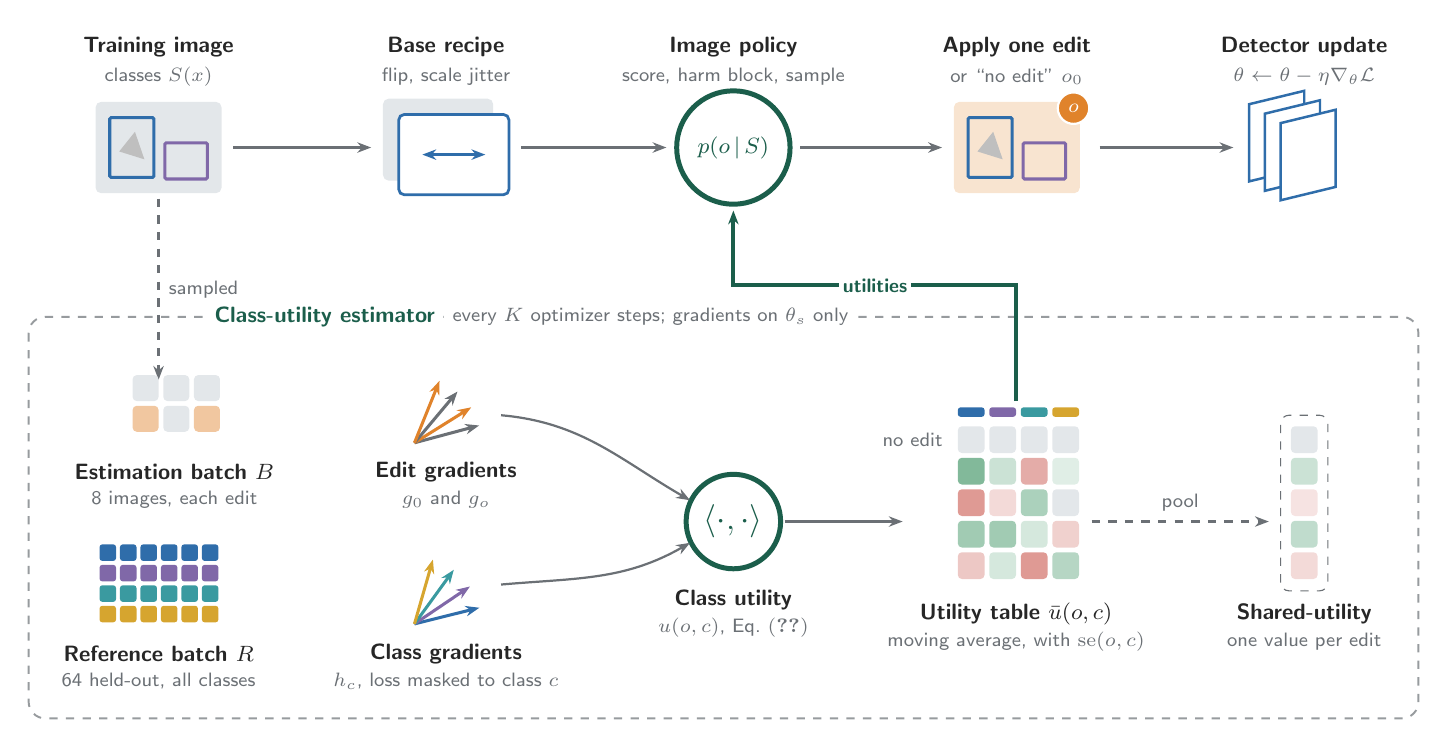
\begin{tikzpicture}[x=1cm, y=1cm, font=\sffamily\footnotesize, >={Stealth[length=5pt]},
  arr/.style={->, draw=cuaArrow, line width=0.8pt},
  lbl/.style={font=\sffamily\footnotesize\bfseries, text=black!85, align=center},
  sub/.style={font=\sffamily\scriptsize, text=cuaText, align=center},
  imgicon/.pic={
    \fill[#1, rounded corners=2pt] (-0.8,-0.58) rectangle (0.8,0.58);
    \draw[cuaBlue, line width=1.1pt, rounded corners=0.5pt] (-0.62,-0.38) rectangle (-0.06,0.38);
    \draw[cuaPurple, line width=1.1pt, rounded corners=0.5pt] (0.08,-0.4) rectangle (0.62,0.06);
    \fill[black!25] (-0.5,-0.05) -- (-0.3,0.2) -- (-0.18,-0.15) -- cycle;},
  imgicon/.default=cuaGrey]
  % ---------------- training step ----------------
  \pic at (0,0) {imgicon=cuaGrey};
  \node[lbl] at (0,1.28) {Training image};
  \node[sub] at (0,0.9) {classes $S(x)$};
  % base recipe
  \fill[cuaGrey, rounded corners=2pt] (2.85,-0.42) rectangle (4.25,0.62);
  \filldraw[fill=white, draw=cuaBlue, line width=1pt, rounded corners=2pt] (3.05,-0.6) rectangle (4.45,0.42);
  \draw[<->, cuaBlue, line width=0.9pt] (3.35,-0.09) -- (4.15,-0.09);
  \node[lbl] at (3.65,1.28) {Base recipe};
  \node[sub] at (3.65,0.9) {flip, scale jitter};
  % image policy
  \filldraw[fill=white, draw=cuaGreen, line width=1.8pt] (7.3,0) circle (0.72);
  \node[text=cuaGreen, font=\footnotesize] at (7.3,0) {$p(o\,|\,S)$};
  \node[lbl] at (7.3,1.28) {Image policy};
  \node[sub] at (7.3,0.9) {score, harm block, sample};
  % edited image
  \pic at (10.9,0) {imgicon=cuaOrange!22};
  \filldraw[fill=cuaOrange, draw=white, line width=0.8pt] (11.62,0.5) circle (0.2);
  \node[text=white, font=\sffamily\scriptsize\bfseries] at (11.62,0.5) {$o$};
  \node[lbl] at (10.9,1.28) {Apply one edit};
  \node[sub] at (10.9,0.9) {or ``no edit'' $o_0$};
  % detector
  \foreach \i in {0,1,2} {
    \filldraw[fill=white, draw=cuaBlue, line width=0.9pt, shift={(14.35+0.2*\i,0.12-0.12*\i)}]
      (-0.5,-0.55) -- (0.2,-0.38) -- (0.2,0.6) -- (-0.5,0.43) -- cycle; }
  \node[lbl] at (14.55,1.28) {Detector update};
  \node[sub] at (14.55,0.9) {$\theta\leftarrow\theta-\eta\nabla_\theta\mathcal{L}$};
  \draw[arr] (0.95,0) -- (2.7,0);
  \draw[arr] (4.6,0) -- (6.45,0);
  \draw[arr] (8.15,0) -- (9.95,0);
  \draw[arr] (11.95,0) -- (13.65,0);
  % ---------------- estimator ----------------
  \draw[cuaText!70, dashed, rounded corners=6pt, line width=0.7pt] (-1.65,-2.15) rectangle (16.0,-7.25);
  \node[anchor=west, fill=white, inner sep=3pt, text=cuaGreen, font=\sffamily\footnotesize\bfseries] (est) at (0.6,-2.15) {Class-utility estimator};
  \node[anchor=west, fill=white, inner sep=3pt, text=cuaText, font=\sffamily\scriptsize] at (est.east) {every $K$ optimizer steps; gradients on $\theta_s$ only};
  \draw[arr, dashed] (0,-0.65) -- node[right, sub]{sampled} (0,-2.95);
  % estimation batch (2x2 tiles, one edited)
  \foreach \c/\x/\y in {cuaGrey/-0.33/-3.22, cuaGrey/0.06/-3.22, cuaOrange!45/-0.33/-3.61, cuaGrey/0.06/-3.61} {
    \fill[\c, rounded corners=1.5pt] (\x,\y) rectangle ++(0.33,0.33); }
  \foreach \c/\x/\y in {cuaGrey/0.45/-3.22, cuaOrange!45/0.45/-3.61} {
    \fill[\c, rounded corners=1.5pt] (\x,\y) rectangle ++(0.33,0.33); }
  \node[lbl] at (0.2,-4.12) {Estimation batch $B$};
  \node[sub] at (0.2,-4.47) {8 images, each edit};
  % edit gradients
  \foreach \a/\c in {15/cuaArrow, 32/cuaOrange, 50/cuaArrow, 68/cuaOrange} {
    \draw[->, \c, line width=1.1pt] (3.25,-3.75) -- ++(\a:0.85); }
  \node[lbl] at (3.65,-4.12) {Edit gradients};
  \node[sub] at (3.65,-4.47) {$g_0$ and $g_o$};
  % reference batch (stratified tiles)
  \foreach \r/\c in {0/cuaBlue, 1/cuaPurple, 2/cuaTeal, 3/cuaGold} {
    \foreach \k in {0,...,5} {
      \fill[\c, rounded corners=1pt] (-0.75+0.26*\k,-5.25-0.26*\r) rectangle ++(0.21,0.21); } }
  \node[lbl] at (0.0,-6.43) {Reference batch $R$};
  \node[sub] at (0.0,-6.78) {64 held-out, all classes};
  % class gradients
  \foreach \a/\c in {14/cuaBlue, 34/cuaPurple, 54/cuaTeal, 74/cuaGold} {
    \draw[->, \c, line width=1.1pt] (3.25,-6.05) -- ++(\a:0.85); }
  \node[lbl] at (3.65,-6.43) {Class gradients};
  \node[sub] at (3.65,-6.78) {$h_c$, loss masked to class $c$};
  % alignment
  \filldraw[fill=white, draw=cuaGreen, line width=1.8pt] (7.3,-4.75) circle (0.6);
  \node[text=cuaGreen, font=\large\bfseries] at (7.3,-4.75) {$\langle\cdot,\cdot\rangle$};
  \node[lbl] at (7.3,-5.75) {Class utility};
  \node[sub] at (7.3,-6.1) {$u(o,c)$, Eq.~\eqref{eq:utility}};
  \draw[arr] (4.35,-3.4) to[out=-5, in=150] (6.75,-4.48);
  \draw[arr] (4.35,-5.55) to[out=5, in=-150] (6.75,-5.02);
  % utility table
  \foreach \k/\c in {0/cuaBlue, 1/cuaPurple, 2/cuaTeal, 3/cuaGold} {
    \fill[\c, rounded corners=1pt] (10.15+0.4*\k,-3.42) rectangle ++(0.34,0.12); }
  \foreach \r/\a/\b/\cc/\d in {
      0/cuaGrey/cuaGrey/cuaGrey/cuaGrey,
      1/cuaPos!60/cuaPos!25/cuaNeg!45/cuaPos!15,
      2/cuaNeg!55/cuaNeg!20/cuaPos!40/cuaGrey,
      3/cuaPos!45/cuaPos!45/cuaPos!20/cuaNeg!25,
      4/cuaNeg!30/cuaPos!20/cuaNeg!55/cuaPos!35} {
    \foreach \k/\c in {0/\a, 1/\b, 2/\cc, 3/\d} {
      \fill[\c, rounded corners=1.5pt] (10.15+0.4*\k,-3.88-0.4*\r) rectangle ++(0.34,0.34); } }
  \node[sub, anchor=east] at (10.08,-3.71) {no edit};
  \node[lbl] at (10.89,-5.92) {Utility table $\bar u(o,c)$};
  \node[sub] at (10.89,-6.27) {moving average, with $\mathrm{se}(o,c)$};
  \draw[arr] (7.95,-4.75) -- (9.45,-4.75);
  % shared variant
  \foreach \r/\c in {0/cuaGrey, 1/cuaPos!25, 2/cuaNeg!15, 3/cuaPos!30, 4/cuaNeg!20} {
    \fill[\c, rounded corners=1.5pt] (14.38,-3.88-0.4*\r) rectangle ++(0.34,0.34); }
  \draw[cuaText, dashed, rounded corners=3pt] (14.25,-5.63) rectangle (14.85,-3.4);
  \node[lbl] at (14.55,-5.92) {Shared-utility};
  \node[sub] at (14.55,-6.27) {one value per edit};
  \draw[arr, dashed] (11.85,-4.75) -- node[above, sub]{pool} (14.1,-4.75);
  % utilities back to the policy
  \draw[->, draw=cuaGreen, line width=1.5pt] (10.89,-3.22) -- (10.89,-1.75) -| (7.3,-0.8);
  \node[text=cuaGreen, font=\sffamily\scriptsize\bfseries, fill=white, inner sep=1.5pt] at (9.1,-1.75) {utilities};
\end{tikzpicture}
\caption{Overview of Class-Utility Augmentation (CUA). Top: in every training step, each image receives the base recipe and then one edit, chosen by the image policy from the classes the image contains; ``no edit'' is always a candidate. Bottom: every $K$ steps, the estimator compares the gradients of the training loss on an edited and an unedited estimation batch with the gradient of each class's loss on a shared reference batch. Their alignment estimates how much each edit helps each class learn (Eq.~\eqref{eq:utility}); the smoothed estimates form the utility table (green: helps, red: hurts, values illustrative) that the policy reads. Shared-utility augmentation pools each row of the table into one value, so every image receives the same preferences; it differs from CUA in nothing else.}
\label{fig:framework}
\end{figure*}

\subsection{Problem Setup}
\label{sec:method_setup}

Let $f_\theta$ be a detector with parameters $\theta$, trained on images annotated with boxes from a set of classes $\mathcal{C}$. A training image $x$ carries annotations $Y=\{(b_j,c_j)\}_{j=1}^{n}$, and we write $S(x)=\{c_1,\dots,c_n\}\subseteq\mathcal{C}$ for the set of classes it contains, so that $|S(x)|\geq 2$ for a multi-class image. Training minimizes the standard detection loss $\mathcal{L}(\cdot\,;\theta)$, which sums classification and box-regression terms over the matched proposals or anchors.

Every training image first receives a base recipe that all compared policies share: a horizontal flip with probability 0.5, followed by isotropic scale jitter with a factor drawn from $[0.8,1.2]$ on a $640\times640$ letterboxed canvas, where a draw that pushes an annotated box out of the canvas is redrawn. The base recipe is never adapted. On top of it, an augmentation policy chooses one edit $o$ from the candidate set $\mathcal{O}\cup\{o_0\}$, where $\mathcal{O}$ is the augmentation menu of the dataset (Table~\ref{tab:menu}) and $o_0$ is the identity, or ``no edit''. We write $T_o$ for the transformation that applies edit $o$ to an image together with its boxes. The menu covers geometric, colour, image-quality, occlusion and composition edits, each at one moderate strength, so the policy controls which edit an image receives rather than how strong that edit is. The task of the policy is to choose $o$ for each image so that the resulting training step benefits the classes the image contains.

\subsection{Estimating Class Utility}
\label{sec:method_estimator}

The quantity CUA needs is the effect that training on an edited image has on what the detector learns about each class. Measuring this effect directly requires training a separate detector for each edit, which is the costly protocol of Section~\ref{sec:measurement}; CUA instead estimates it during training from a single gradient step. Consider one stochastic gradient step with learning rate $\eta$ on a batch $B$ of training images. If the batch is edited by $o$, the step changes the parameters by $-\eta\,g_o$ with $g_o=\nabla_\theta\mathcal{L}(T_o(B);\theta)$, and if it is left unedited, by $-\eta\,g_0$ with $g_0=\nabla_\theta\mathcal{L}(B;\theta)$. Let $\mathcal{L}_c(R;\theta)$ be the loss of class $c$ on a held-out batch $R$ of images, restricted to the proposals or anchors matched to class-$c$ ground truth, and let $h_c=\nabla_\theta\mathcal{L}_c(R;\theta)$. To first order, the step on the edited batch reduces this loss by $\eta\langle g_o,h_c\rangle$ and the step on the unedited batch by $\eta\langle g_0,h_c\rangle$. We define the class utility of edit $o$ for class $c$ as the difference between the two reductions, normalized by the current loss of the class:
\begin{equation}
u(o,c)=\frac{\eta\,\langle g_o-g_0,\;h_c\rangle}{\mathcal{L}_c(R;\theta)+\delta},
\label{eq:utility}
\end{equation}
with $\delta=0.01$. A positive $u(o,c)$ means that a step on the edited batch moves the detector further toward a lower loss for class $c$ than a step on the unedited batch would, so the edit currently teaches the class something useful; a negative value means that the edit pulls the learning of $c$ in the wrong direction. By construction, $u(o_0,c)=0$ for every class. The normalization by $\mathcal{L}_c$ makes utilities comparable across classes whose losses differ in scale, so that no class dominates the score of an image merely because its loss is large. Eq.~\eqref{eq:utility} is the first-order influence estimate of TracIn~\cite{pruthi2020tracin}, applied here to a pair of edited and unedited batches rather than to one training example, and to a separate reference loss for each class rather than to one test loss. Like TracIn, it ignores optimizer momentum and higher-order terms, and it predicts the effect of one step rather than of training to convergence; Section~\ref{sec:measurement} provides the measurements against which this approximation is checked.

The held-out images come from a \emph{reference set} of about 1,000 training images that are removed from optimization in every compared policy and are used only by the estimator, so that the utilities reflect images the detector has not trained on. Every $K$ optimizer steps, CUA draws an estimation batch $B$ of eight training images and one reference batch $R$ of 64 reference images, stratified so that every class appears in $R$ at least once. It computes $g_0$ on the unedited batch and $g_o$ on each edited version, using the same random draws for all of them so that the comparison is paired. All class gradients come from a single forward pass over $R$: for each class $c$, $\mathcal{L}_c(R;\theta)$ is the loss restricted to the proposals (Faster R-CNN) or anchors (RetinaNet) matched to class-$c$ boxes in $R$, and one backward pass gives $h_c$. Because all classes share one reference batch, the number of reference images does not grow with the number of classes.

Gradients are taken only with respect to a parameter subset $\theta_s$: the box head and box predictor together with the top feature-pyramid level for Faster R-CNN, and the classification and regression heads together with the top feature-pyramid level for RetinaNet. These parameters are closest to the class decision, which is where a class-specific effect of an edit is expressed. All other parameters are frozen during estimation, so the backbone and the remaining pyramid layers run without gradients and each per-class backward pass is cheap; the estimator only reads gradients and never changes the model. Estimation passes run in single precision even though training uses mixed precision, because in half precision the summed class losses can overflow and produce non-finite utilities.

A single estimate is noisy, because it rests on eight training images and one draw of each edit. CUA therefore smooths the estimates with exponential moving averages of the utility and of its squared deviation,
\begin{align}
\bar u(o,c)&\leftarrow\beta\,\bar u(o,c)+(1-\beta)\,u(o,c),\label{eq:ema}\\
v(o,c)&\leftarrow\beta\,v(o,c)+(1-\beta)\bigl(u(o,c)-\bar u(o,c)\bigr)^2,\label{eq:var}
\end{align}
with $\beta=0.9$; the first estimate of a cell initializes $\bar u(o,c)$, and $v(o,c)$ starts at zero. CUA takes $\mathrm{se}(o,c)=\sqrt{v(o,c)\,(1-\beta)/(1+\beta)}$ as the standard error of the average, since $(1-\beta)/(1+\beta)$ is the variance of an exponential moving average of independent estimates relative to that of a single estimate. Estimation starts after the first training epoch; until then no utilities exist, and the policy samples uniformly from $\mathcal{O}\cup\{o_0\}$. Because the table is refreshed throughout training, the edit that a class prefers can change as the detector improves.

\subsection{Choosing an Edit for Each Image}
\label{sec:method_policy}

The image policy turns the utility table into one decision per image. For an image with class set $S=S(x)$, CUA scores each candidate edit by the average utility of the classes present,
\begin{equation}
s(o\mid S)=\frac{1}{|S|}\sum_{c\in S}w_c\,\bar u(o,c),
\label{eq:score}
\end{equation}
with equal class weights $w_c=1$. Averaging over the classes in the image, rather than over all classes, is what makes the decision depend on the image: an image that contains only potholes is scored by the pothole entries of the table, whereas an image that contains a crack and a pothole is scored by both. Since the identity scores $s(o_0\mid S)=0$, an edit is preferred to leaving the image unchanged only when its average utility over the classes present is positive.

An average can still hide a loss for one of the classes, which is precisely the failure CUA is designed to avoid. Before sampling, CUA therefore removes every edit that is reliably harmful to at least one class in the image, and keeps the allowed set
\begin{equation}
\mathcal{A}(S)=\Bigl\{o:\ \min_{c\in S}\bigl[\bar u(o,c)+1.64\,\mathrm{se}(o,c)\bigr]\geq 0\Bigr\},
\label{eq:harm}
\end{equation}
where $o$ ranges over $\mathcal{O}\cup\{o_0\}$. The set excludes an edit whenever its utility for a present class is negative at one-sided 95\% confidence. A cell enters the harm block only after it has been estimated three times, so that its standard error rests on more than one estimate. The identity is never excluded, because its utility and standard error are zero, so $\mathcal{A}(S)$ is never empty. CUA then samples the edit from
\begin{equation}
p(o\mid S)=(1-\varepsilon)\,\frac{\exp\bigl(s(o\mid S)/\tau\bigr)}{Z(S)}+\frac{\varepsilon}{|\mathcal{A}(S)|},
\label{eq:sampling}
\end{equation}
for $o\in\mathcal{A}(S)$, where $Z(S)=\sum_{o'\in\mathcal{A}(S)}\exp\bigl(s(o'\mid S)/\tau\bigr)$ normalizes the softmax, $\varepsilon=0.1$, and the temperature $\tau$ is the standard deviation of the current scores over $\mathcal{A}(S)$, floored at $10^{-6}$. Tying $\tau$ to the spread of the scores keeps the distribution unchanged when all utilities shrink or grow together, as they do when the loss falls during training. The uniform term keeps some diversity among the allowed edits, which limits the damage when an estimate is wrong.

Two cases complete the policy. Images that contain no annotated object have an empty class set; in every compared policy, such an image receives either the identity or a uniformly sampled edit, each with probability 0.5, so the treatment of background-only images does not differ between methods. Mosaic combines four images; CUA chooses it from the class set of the anchor image, and the other three tiles are drawn uniformly from the training set.

\subsection{Shared-Utility Augmentation}
\label{sec:method_shared}

To isolate the contribution of class information, we define a counterpart that differs from CUA in that respect alone. Shared-utility augmentation runs the same estimator and the same policy, but it pools the instantaneous estimates over all classes, $u_{\mathrm{sh}}(o)=\frac{1}{|\mathcal{C}|}\sum_{c\in\mathcal{C}}u(o,c)$, smooths them as in Eq.~\eqref{eq:ema}, and applies the harm block of Eq.~\eqref{eq:harm} to the pooled estimate and its standard error. Every image therefore receives the same edit preferences, whichever classes it contains. Because the estimator, reference set, sampling rule and settings are shared, a difference in accuracy between CUA and shared-utility augmentation can be attributed to the use of per-class utilities.

\subsection{Computational Cost}
\label{sec:method_cost}

CUA adds no policy network, no search phase before training and no training images; its only cost is the periodic estimation step. Each estimation step runs $(|\mathcal{O}|+1)\cdot 8+64$ image forward passes, for the unedited and edited estimation batches and the reference batch, and $|\mathcal{O}|+1+|\mathcal{C}|$ backward passes through $\theta_s$ only, and it is repeated every $K$ optimizer steps. Because the reference batch is shared by all classes, the number of forward passes does not depend on the number of classes; the classes enter only through backward passes restricted to $\theta_s$, which are small compared with a forward pass through the backbone. Our target was an estimator overhead below 20\%. On RDD2022 with Faster R-CNN and $K=200$, one estimation step takes about 8.6\,s on an NVIDIA A10, and the estimator accounts for about 15\% of the wall-clock time of an epoch including validation, or about 18\% on top of the rest of the epoch.

\section{Measuring Class-Specific Augmentation Effects}
\label{sec:measurement}

CUA can help only if classes respond differently to the same edit, and its estimates are useful only if they track how classes actually respond. We therefore measure these responses directly, with controlled training runs that do not involve CUA. The measurements serve three purposes: they test whether augmentation effects in detection depend on the class, they provide the reference against which the class utilities of Section~\ref{sec:method} are checked, and they define the measured-effect policy used as a baseline in Section~\ref{sec:setup}. All measurements use the datasets, detectors and training recipe of Section~\ref{sec:setup}, and all are evaluated on the validation split.

\subsection{Edit-Wise Measurement Study}
\label{sec:measure_editwise}

The edit-wise study measures the effect of each edit on each class by training with one edit at a time. Training a full detector for every edit, dataset, detector and seed would be prohibitively expensive, so the study branches short training runs from a shared starting point. For each dataset, detector and seed, we first train a warm checkpoint with the base recipe for three epochs. From this checkpoint, we continue training for three further epochs in $|\mathcal{O}|+1$ branches: one with the base recipe alone, and one for each valid edit $o$, in which $o$ is applied to the whole image with probability 0.5 after the base recipe. The learning rate remains at its base value for the first two continuation epochs and is reduced tenfold for the last. All branches share the warm checkpoint and its optimizer state, the order of the training images, the base-recipe draws and the random draw that decides whether an edit is applied, so any two branches differ only in the edit itself. For edit $o$, class $c$ and seed $k$, the measured effect is the change in validation AP50 at the end of the continuation,
\begin{equation}
\Delta_{o,c,k}=\mathrm{AP50}_c(o,k)-\mathrm{AP50}_c(\mathrm{base},k),
\label{eq:delta}
\end{equation}
and averaging over seeds gives the edit--class effect table $\bar\Delta(o,c)$. The study covers the three datasets, both detector families and seeds $\{0,1,2\}$, for a total of 258 training runs including the warm checkpoints.

\subsection{Testing Whether Effects Depend on the Class}
\label{sec:measure_tests}

A difference between two classes in Eq.~\eqref{eq:delta} can arise from training noise as well as from a genuine class dependence, so we test the dependence statistically for each dataset and detector. We fit the per-seed effects with the linear model
\begin{equation}
\Delta_{o,c,k}=\mu+\alpha_k+\beta_o+\gamma_c+(\alpha\gamma)_{k,c}+(\beta\gamma)_{o,c}+e_{o,c,k}
\label{eq:anova}
\end{equation}
and compare it, with an $F$-test, against the reduced model without the edit$\times$class term $(\beta\gamma)_{o,c}$. The seed$\times$class term is required because all effects for a given seed and class are computed against the same base branch and therefore share its noise; the term absorbs this shared component exactly. A significant edit$\times$class term means that the effect of an edit depends on the class beyond what the average effect of the edit and the average sensitivity of the class explain. To locate the edits responsible, we then test each edit separately, comparing the model $\Delta_{o,c,k}=\mu+\alpha_k+\gamma_c+e_{c,k}$ with the same model without the class term, and correct the resulting $p$-values across edits with the Holm procedure~\cite{holm1979}. We conclude that the effect of edits depends on the class when the edit$\times$class term is significant at the 5\% level. To describe individual cells, we also count, for each edit, the classes whose effect has the same sign in all three seeds. A cell without any true effect has the same sign in all three seeds with probability $1/4$, so these counts describe the table rather than test it; inference rests on the interaction test and the Holm-corrected contrasts.

\subsection{Agreement Between Short and Full Training}
\label{sec:measure_proxy}

The short continuations measure the effect of an edit early in training, whereas CUA and the compared policies train for the full schedule. To check that the short runs rank edits as full training would, we train the base recipe and four edits for the full schedule on RDD2022 with Faster R-CNN and one seed, choosing the edits to span the ranking of the edit-wise study: the best, the worst and two from the middle. Agreement is measured by the Spearman rank correlation between the seed-averaged short-run effects $\bar\Delta(o,c)$ and the full-run effects over the shared edit--class cells, with a 95\% bootstrap interval from 2,000 resamples of the cells. If the correlation is below 0.5, we treat the short-run effects as indicative of direction only, and the measured-effect policy uses full-run effects wherever they are available.

\section{Experimental Setup}
\label{sec:setup}

\subsection{Datasets}
\label{sec:setup_data}

We evaluate on three domains that differ in how their classes are defined and how often they co-occur (Table~\ref{tab:datasets}). RDD2022~\cite{arya2024rdd} contains road images from several countries with four damage classes: longitudinal cracks (D00), transverse cracks (D10), alligator cracks (D20) and potholes (D40). We use a fixed split of 26,863 training, 5,760 validation and 5,760 test images, in which exact duplicates and perceptually similar images are always assigned to the same partition. dacl10k~\cite{flotzinger2024dacl10k} contains close-up bridge-inspection images with polygon annotations of damage and bridge components. Because the official download is no longer available, we use its public FiftyOne export~\cite{voxel51dacl10k}, which contains 8,922 images under a \todo{confirm licence: CC BY-NC 4.0 or CC BY 4.0} licence. Its 1,012 official test images carry no labels and are discarded, so that unlabelled images are never treated as damage-free, which leaves 7,910 labelled images. We keep the damage classes only, convert each annotated polygon into one box spanning all of its rings and clipped to the image, and drop degenerate polygons. Since the official splits are not available with labels, we group the labelled images by near-duplicate hashing and divide the groups 70/15/15 into training, validation and test partitions. PASCAL VOC~\cite{everingham2010voc} provides 20 everyday object classes; we train on the VOC2007 and VOC2012 trainval sets, from which 10\% of the images are held out for validation, and test on VOC2007 test. Objects marked difficult are excluded from the training targets and treated as ignore regions in evaluation.

\begin{table}[t]
\caption{Datasets, Splits and Co-Occurrence of Classes}
\label{tab:datasets}
\centering
\footnotesize
\setlength{\tabcolsep}{3pt}
\begin{tabular}{@{}lcccccc@{}}
\toprule
\textbf{Dataset} & \textbf{Classes} & \textbf{Train} & \textbf{Ref.} & \textbf{Val} & \textbf{Test} & \textbf{Multi-class} \\
\midrule
RDD2022~\cite{arya2024rdd} & 4 & \todo{n} & \todo{n} & 5,760 & 5,760 & 35\% \\
dacl10k~\cite{flotzinger2024dacl10k} & 12 & 4,609 & 1,000 & 1,160 & 1,141 & 75\% \\
PASCAL VOC~\cite{everingham2010voc} & 20 & 13,694 & 1,206 & 1,651 & 4,952 & 35\% \\
\bottomrule
\end{tabular}
\vspace{2pt}

\parbox{\columnwidth}{\footnotesize Train excludes the reference set (Ref.), which only the class-utility estimator uses. Multi-class: share of object-bearing training images that contain two or more classes.}
\end{table}

\subsection{Data Gates and Reference Set}
\label{sec:setup_gates}

Three checks with fixed thresholds run once on each dataset before any training. First, because CUA addresses images that contain several classes, a dataset is used only if at least 20\% of its object-bearing training images contain two or more classes. Second, a dacl10k class is kept only if it has at least 300 training boxes and no more than half of its boxes cover more than half of the image; the first condition removes classes too rare to evaluate reliably, and the second removes region-like classes that a box describes poorly. This gate uses the training partition only. It keeps 12 of the 13 damage classes, namely Crack, Wetspot, Efflorescence, Rust, Rockpocket, Hollowareas, Cavity, Spalling, Graffiti, Weathering, Restformwork and ExposedRebars, and excludes alligator cracks (ACrack), which have 282 training boxes. Third, we screen for near-duplicate images with 64-bit difference hashes at a Hamming distance of at most 4. In dacl10k, each group of near duplicates is kept within one partition. PASCAL VOC keeps its official partitions so that results remain comparable with other work; the screen finds 20 training--test and 2 validation--test pairs, under 0.5\% of the 4,952 test images, which we report and do not remove. All three datasets pass the co-occurrence gate, with 35\% of object-bearing training images containing two or more classes in RDD2022 and PASCAL VOC and 75\% in dacl10k.

From each training partition we then remove a reference set of about 1,000 images (Table~\ref{tab:datasets}), chosen in whole near-duplicate groups so that each class has at least 100 objects where possible. The reference set is excluded from optimization in every compared policy, including the base recipe, so that all policies train on identical data. The remaining partitions have fixed roles: the training images are used for optimization, the reference set only for the class-utility estimates, the validation set for the measurements of Section~\ref{sec:measurement}, for tuning and for checkpoint selection, and the test set for the final comparison, which is evaluated once after all settings are fixed.

\subsection{Detectors and Training}
\label{sec:setup_training}

We use two detector families: Faster R-CNN~\cite{ren2017faster} and RetinaNet~\cite{lin2017focal}, both with a ResNet-50 feature pyramid backbone. Both start from COCO-pretrained torchvision weights, with all backbone stages trainable and batch-normalization statistics frozen. Images are letterboxed to $640\times640$ pixels with padding value 114. Training uses stochastic gradient descent with momentum 0.9, weight decay $5\times10^{-4}$, a batch size of four and a base learning rate of 0.0025, reached by a linear warm-up over 1,000 iterations from $0.001$ times that value; the learning rate is reduced tenfold after 60\% of the epochs and a hundredfold after 80\%, and training uses mixed precision. At inference, detections are kept above a score of 0.001 after non-maximum suppression at IoU 0.5, with at most 100 per image. Each run is validated after every epoch, and the checkpoint with the highest validation macro AP50 is the one evaluated on the test set. Seeds $\{0,1,2\}$ are shared across policies and fix the initialization of the new heads, the order of the training images and the augmentation draws.

The number of epochs is fixed for each dataset before policies are compared, from a base-recipe run at a candidate budget of 20 epochs for RDD2022 and PASCAL VOC and 30 for dacl10k. A budget is accepted if validation macro AP50 at the final epoch exceeds its value at the first epoch at the final learning rate by less than 0.3 points; otherwise it is extended by 50\% and checked again. This rule replaced our original one after the first RDD2022 run. The original rule compared the final epoch with the epoch at 80\% of training, which is the last epoch before the final learning-rate reduction, so it measured the jump caused by that reduction rather than whether training had levelled off. Under the rule used, all three candidate budgets are accepted: 20 epochs for RDD2022 (51.05 against 50.96 AP50), 20 epochs for PASCAL VOC (81.57 against 81.59) and 30 epochs for dacl10k, whose validation AP50 stays flat near 20.0 over its last six epochs.

The settings of CUA were fixed before the comparison by a small validation study on RDD2022 with Faster R-CNN, seed 0 and the full schedule. Each setting is scored by validation macro AP50 averaged over the four epochs at the final learning rate, and its overhead is the share of epoch wall time spent in the estimator. Before reading the results, we required a setting to gain at least 0.5 AP50 over the default and to keep the overhead at or below 20\% in order to replace it. No setting met this bar (Table~\ref{tab:tuning}): the largest gain, 0.24 AP50, came from $K=100$, whose overhead of 26.7\% also exceeds the limit. We therefore use $K=200$, the box head with the top feature-pyramid level as $\theta_s$, and $\varepsilon=0.1$ for all datasets and detectors. Across these settings the validation score varied by at most 0.24 AP50 on one seed, so within this range the choice has little effect that a single run can detect.

\begin{table}[t]
\caption{Choice of Estimator Settings on Validation (RDD2022, Faster R-CNN, One Seed)}
\label{tab:tuning}
\centering
\footnotesize
\setlength{\tabcolsep}{4pt}
\begin{tabular}{@{}lcc@{}}
\toprule
\textbf{Setting} & \textbf{Val.\ AP50} & \textbf{Overhead} \\
\midrule
Default ($K{=}200$, head+FPN, $\varepsilon{=}0.1$) & 49.61 & 15.3\% \\
$K=100$ & 49.84 & 26.7\%$^{\ast}$ \\
$K=400$ & 49.66 & 8.2\% \\
$\theta_s$ = box head only & 49.81 & 13.0\% \\
$\varepsilon=0.05$ & 49.78 & 15.0\% \\
$\varepsilon=0.2$ & 49.78 & 15.2\% \\
\bottomrule
\end{tabular}
\vspace{2pt}

\parbox{\columnwidth}{\footnotesize Score: mean over the four epochs at the final learning rate. Overhead: estimator share of epoch wall time. $^{\ast}$Above the 20\% limit.}
\end{table}

\subsection{Augmentation Menu}
\label{sec:setup_menu}

Table~\ref{tab:menu} lists the edits and their strengths. Each edit has one strength range, from which a value is drawn every time the edit is applied. Geometric edits transform the boxes together with the image, with a rotated box replaced by the axis-aligned hull of its rotated corners; a draw that pushes a box out of the canvas is redrawn up to ten times, after which the image is left unedited. The validity of each edit is fixed per dataset before training. Vertical flips are excluded for RDD2022, whose images are taken from a vehicle with the road always below the horizon, and for PASCAL VOC, whose upside-down scenes are not label-preserving in practice. Rotation is limited to $\pm10^\circ$ on every dataset, because larger rotations of road images would turn longitudinal cracks into transverse ones. Copy-paste augmentation is not included, because RDD2022 provides no instance masks.

\begin{table}[t]
\caption{Augmentation Menu and Validity per Dataset}
\label{tab:menu}
\centering
\footnotesize
\setlength{\tabcolsep}{3pt}
\begin{tabularx}{\columnwidth}{@{}llYccc@{}}
\toprule
\textbf{Family} & \textbf{Edit} & \textbf{Strength} & \textbf{RDD} & \textbf{VOC} & \textbf{dacl} \\
\midrule
Geometric & Translation & up to $\pm10\%$ of the canvas per axis & $\checkmark$ & $\checkmark$ & $\checkmark$ \\
 & Rotation & $\pm10^\circ$ & $\checkmark$ & $\checkmark$ & $\checkmark$ \\
 & Vertical flip & -- & -- & -- & $\checkmark$ \\
Colour & Brightness & factor in $[0.7,1.3]$ & $\checkmark$ & $\checkmark$ & $\checkmark$ \\
 & Contrast & factor in $[0.7,1.3]$ & $\checkmark$ & $\checkmark$ & $\checkmark$ \\
 & Saturation & factor in $[0.5,1.5]$ & $\checkmark$ & $\checkmark$ & $\checkmark$ \\
 & Hue & shift up to $\pm0.05$ of the hue circle & $\checkmark$ & $\checkmark$ & $\checkmark$ \\
Image quality & Gaussian blur & $\sigma\in[0.5,1.5]$ px & $\checkmark$ & $\checkmark$ & $\checkmark$ \\
 & Gaussian noise & $\sigma=0.03$ of the intensity range & $\checkmark$ & $\checkmark$ & $\checkmark$ \\
 & JPEG compression & quality in $[30,60]$ & $\checkmark$ & $\checkmark$ & $\checkmark$ \\
 & Sharpening & factor in $[1.5,2.5]$ & $\checkmark$ & $\checkmark$ & $\checkmark$ \\
Occlusion & Random erasing~\cite{zhong2020erasing} & 2--10\% of the canvas, noise-filled, at most 50\% of any box & $\checkmark$ & $\checkmark$ & $\checkmark$ \\
Composition & Mosaic~\cite{bochkovskiy2020yolov4} & $2\times2$ tiles at half scale; boxes less than 30\% visible dropped & $\checkmark$ & $\checkmark$ & $\checkmark$ \\
\midrule
\multicolumn{3}{@{}l}{Valid edits} & 12 & 12 & 13 \\
\bottomrule
\end{tabularx}
\end{table}

\subsection{Compared Policies}
\label{sec:setup_policies}

We compare five policies, all applied on top of the base recipe and all trained on the same data, schedule and seeds. The \emph{base recipe} applies no further edit. \emph{Uniform augmentation} samples one edit uniformly from $\mathcal{O}\cup\{o_0\}$ for every image, in the manner of TrivialAugment~\cite{muller2021trivial}, and measures the value of the menu without any choice. The \emph{measured-effect policy} uses the policy of Section~\ref{sec:method_policy} with the class utilities replaced by the measured effects $\bar\Delta(o,c)$ of Section~\ref{sec:measurement}, and their standard errors by the standard deviation of $\Delta_{o,c,k}$ over the three seeds divided by $\sqrt{3}$, with the same one-sided harm rule; it is fixed throughout training and shows what class-specific choices achieve when the effects are measured offline rather than estimated online. \emph{Shared-utility augmentation} (Sec.~\ref{sec:method_shared}) and \emph{CUA} complete the comparison.

Ablations on the validation sets of RDD2022 and dacl10k, with Faster R-CNN and three seeds, remove or replace one component of CUA at a time: the harm block of Eq.~\eqref{eq:harm}; the identity candidate $o_0$; and equal class weights, replaced by weights $w_c$ inversely proportional to the current validation AP of each class.

\subsection{Metrics and Statistics}
\label{sec:setup_metrics}

The primary metric is test macro AP50: average precision at an IoU threshold of 0.5, computed with the COCO evaluation protocol~\cite{lin2014coco} and averaged over the classes that have at least one test object. Secondary metrics are AP50:95, per-class AP50, AP for small, medium and large objects, and, for RDD2022, the fraction of object-free test images that receive at least one detection above confidence \todo{threshold}. We also report the wall-clock overhead of the estimator.

Every policy is trained with the same three seeds, so all comparisons are paired, and we report the mean and standard deviation over seeds. For the difference between two policies, we compute two 95\% intervals: a paired $t$ interval over seeds, and a paired image-level bootstrap~\cite{efron1979} that draws 1,000 resamples of the test images, uses the same images for every policy and seed, and averages the per-seed differences. We claim a difference only when both intervals exclude zero in the claimed direction. The primary comparison is CUA against shared-utility augmentation on test macro AP50; we also compare CUA with the best simple baseline, which is the base recipe or uniform augmentation, whichever has the higher mean test macro AP50. We report each of the six dataset--detector comparisons separately and apply no correction across them. If the interval of the primary comparison spans zero and is wider than 1.0 AP50, both policies are trained with two further seeds. The test set is used once, after all settings are fixed. To test whether CUA estimates what it is meant to estimate, we compute the Spearman correlation between the class utilities averaged over training and the measured effects $\bar\Delta(o,c)$, with a bootstrap interval over edit--class cells.

\subsection{Implementation}
\label{sec:setup_impl}

All methods are implemented in PyTorch~\cite{paszke2019pytorch} 2.3 with torchvision 0.18 and trained on single NVIDIA A10 GPUs. Every run uses the same evaluation code, based on pycocotools. The complete study used \todo{measured GPU-hours} GPU-hours, of which the class-utility estimator accounted for \todo{share}.


\section{Results}
\label{sec:results}

\subsection{Do Augmentation Effects Depend on the Class?}
\label{sec:results_measurement}

Table~\ref{tab:interaction} reports the edit$\times$class interaction test of Section~\ref{sec:measure_tests} for the six dataset--detector pairs, and Fig.~\ref{fig:heatmaps} shows the per-class effect of every edit from which the tests are computed.

\begin{table}[t]
\caption{Edit$\times$Class Interaction Tests in the Edit-Wise Measurement Study (Validation, Three Seeds)}
\label{tab:interaction}
\centering
\footnotesize
\setlength{\tabcolsep}{2.6pt}
\begin{tabular}{@{}llccccl@{}}
\toprule
\textbf{Dataset} & \textbf{Det.} & $|\mathcal{C}|$ & $|\mathcal{O}|$ & $F$ (df) & $p$ & \textbf{Holm} \\
\midrule
RDD2022 & F & 4 & 12 & 3.73 (33, 88) & $4.5\times10^{-7}$ & -- \\
RDD2022 & R & 4 & 12 & 0.79 (33, 88) & 0.77 & -- \\
VOC & F & 20 & 12 & 1.60 (209, 440) & $2.4\times10^{-5}$ & -- \\
VOC & R & 20 & 12 & 1.91 (209, 440) & $1.0\times10^{-8}$ & mosaic \\
dacl10k & F & 12 & 13 & 2.52 (132, 288) & $4.1\times10^{-11}$ & mosaic, contrast \\
dacl10k & R & 12 & 13 & 1.06 (132, 288) & 0.34 & -- \\
\bottomrule
\end{tabular}
\vspace{2pt}

\parbox{\columnwidth}{\footnotesize Det.: F = Faster R-CNN, R = RetinaNet. Holm: edits whose per-edit class contrast remains significant at 5\% after Holm correction across edits.}
\end{table}

\begin{figure*}[t]
\centering
\includegraphics[width=\textwidth]{figures/measurement_heatmaps.pdf}
\caption{Per-class effect of each edit in the edit-wise measurement study (validation, mean over three seeds). Each cell is the change in AP50 when the edit is added to the base recipe; green cells gain and red cells lose. A dot marks a cell whose change has the same sign in all three seeds, which also happens for a quarter of cells without any true effect. Panel titles give the edit$\times$class interaction test of Table~\ref{tab:interaction}, in green when significant at 5\%. Rows whose colour changes sign within a panel are edits whose effect depends on the class; uniformly red rows, such as mosaic on RDD2022, are edits that cost every class.}
\label{fig:heatmaps}
\end{figure*}

\noindent\textbf{The effect of an edit depends on the class.} With Faster R-CNN, the edit$\times$class interaction is significant in all three domains: on RDD2022 ($F(33,88)=3.73$, $p=4.5\times10^{-7}$), on PASCAL VOC ($F(209,440)=1.60$, $p=2.4\times10^{-5}$) and on dacl10k ($F(132,288)=2.52$, $p=4.1\times10^{-11}$). With RetinaNet, it is significant on PASCAL VOC only ($F(209,440)=1.91$, $p=1.0\times10^{-8}$). In four of the six dataset--detector pairs, therefore, how much an edit changes AP50 depends on which class is measured, beyond what the average effect of the edit and the average sensitivity of the class explain.

\noindent\textbf{Two edits carry the dependence that survives correction.} When each edit is tested on its own and the results are corrected across edits, two edits remain significant on dacl10k with Faster R-CNN, mosaic ($p_{\mathrm{Holm}}=0.0003$) and contrast ($p_{\mathrm{Holm}}=0.002$), and one on PASCAL VOC with RetinaNet, mosaic ($p_{\mathrm{Holm}}<0.001$). Contrast on dacl10k is the clearest case of an edit that helps some classes and hurts others: its effect is positive in all three seeds for Crack and Hollowareas, and negative in all three seeds for Efflorescence, Rust, Graffiti, Weathering, Restformwork and ExposedRebars. The classes it hurts include the colour-defined defects named in Section~\ref{sec:intro}, rust and efflorescence, although the study does not test why. Mosaic on PASCAL VOC with RetinaNet is a different case: the classes differ in how much it helps rather than in whether it helps. It raises AP50 by 1.82 on average, its effect is positive in all three seeds for 16 of the 20 classes, and its class means span 7.6 AP50.

\noindent\textbf{Opposite effects on single classes are common but mostly within noise.} Beyond these two edits, several edits have effects of opposite sign on different classes in all three seeds. On dacl10k with Faster R-CNN, mosaic is positive for three classes and negative for six, and sharpening positive for three and negative for two; on PASCAL VOC with Faster R-CNN, rotation is positive for four classes and negative for three, and sharpening and hue are each positive for three and negative for three; on dacl10k with RetinaNet, vertical flip is positive for three and negative for three, although that pair shows no significant interaction. These counts must be read with care. A cell without any true effect has the same sign in all three seeds with probability $1/4$, so with 20 classes about 2.5 such cells per edit and direction are expected from seed noise alone, and the PASCAL VOC counts are of that size. The interaction tests, not these counts, carry the inference.

\begin{table}[t]
\caption{Mean Change in Validation AP50 over Classes for Each Edit (Edit $-$ Base, Three Seeds)}
\label{tab:mean_effects}
\centering
\footnotesize
\setlength{\tabcolsep}{3.2pt}
\begin{tabular}{@{}lrrrrrr@{}}
\toprule
 & \multicolumn{2}{c}{\textbf{RDD2022}} & \multicolumn{2}{c}{\textbf{VOC}} & \multicolumn{2}{c}{\textbf{dacl10k}} \\
\cmidrule(lr){2-3}\cmidrule(lr){4-5}\cmidrule(l){6-7}
\textbf{Edit} & F & R & F & R & F & R \\
\midrule
Mosaic & $-$3.55 & $-$2.93 & $-$0.85 & +1.82 & $-$0.64 & $-$0.51 \\
Blur & $-$1.27 & $-$0.73 & $-$0.34 & $-$0.59 & $-$0.27 & $-$0.02 \\
Rotation & $-$0.75 & $-$0.56 & $-$0.10 & $-$0.06 & +0.05 & +0.03 \\
JPEG & $-$0.67 & $-$0.33 & $-$0.29 & $-$0.19 & $-$0.36 & $-$0.05 \\
Noise & $-$0.52 & $-$0.93 & $-$0.32 & $-$0.21 & $-$0.23 & +0.13 \\
Translation & $-$0.44 & $-$0.63 & $-$0.22 & $-$0.09 & $-$0.03 & +0.18 \\
Contrast & $-$0.29 & +0.08 & $-$0.32 & $-$0.10 & $-$0.12 & +0.07 \\
Random erasing & $-$0.25 & $-$0.51 & $-$0.37 & $-$0.12 & $-$0.24 & +0.04 \\
Hue & $-$0.21 & $-$0.31 & $-$0.10 & $-$0.04 & $-$0.16 & $-$0.10 \\
Brightness & $-$0.17 & $-$0.70 & $-$0.26 & $-$0.05 & $-$0.01 & +0.13 \\
Saturation & $-$0.01 & $-$0.24 & $-$0.13 & $-$0.03 & $-$0.10 & $-$0.08 \\
Sharpening & +0.14 & $-$0.39 & $-$0.08 & $-$0.17 & $-$0.01 & +0.35 \\
Vertical flip & -- & -- & -- & -- & $-$0.31 & +0.19 \\
\bottomrule
\end{tabular}
\vspace{2pt}

\parbox{\columnwidth}{\footnotesize F: Faster R-CNN; R: RetinaNet. --: edit not valid for the dataset.}
\end{table}

\noindent\textbf{Most edits cost a little in the short run, and mosaic stands out.} Averaged over classes, most edits lower validation AP50 slightly in the three-epoch continuation, and no edit raises AP50 consistently for all classes of a dataset (Table~\ref{tab:mean_effects}). Mosaic is the exception in both directions. It is strongly negative on RDD2022 ($-3.55$ AP50 with Faster R-CNN and $-2.93$ with RetinaNet), mildly negative on dacl10k ($-0.64$ and $-0.51$) and negative on PASCAL VOC with Faster R-CNN ($-0.85$), but positive on PASCAL VOC with RetinaNet ($+1.82$). Because the continuation lasts only three epochs, these averages describe the early effect of an edit; the next paragraph examines how far they carry over to full training.

\noindent\textbf{Short runs agree moderately with full training.} For RDD2022 with Faster R-CNN, the base recipe and four edits retrained with the full 20-epoch schedule give a Spearman correlation of $\rho=0.56$ between short-run and full-run per-class effects over 16 edit--class cells, with a 95\% bootstrap interval of $[0.04,\,0.86]$. The correlation passes the threshold of 0.5 set before the run, but the interval is wide. We therefore treat the signs of the short-run effects as moderately reliable and their sizes as indicative only.

\noindent\textbf{RetinaNet shows no class dependence on RDD2022 and dacl10k.} For these two pairs the interaction is not significant ($F=0.79$, $p=0.77$ and $F=1.06$, $p=0.34$), and the differences between classes are of the size expected from seed-to-seed variation. We report this as found. One possibility, which this study does not test, is that three epochs are too few for class differences to appear in RetinaNet's dense head; the agreement check above covers Faster R-CNN only.

Together, these results support the premise of CUA for Faster R-CNN in all three domains and for RetinaNet on PASCAL VOC. For RetinaNet on RDD2022 and dacl10k they do not, and in those two settings CUA is expected to perform like shared-utility augmentation.

\subsection{Does CUA Exploit Class Dependence?}
\label{sec:results_comparison}

\todo{Section VI.B is written when the policy comparison finishes: main comparison (Table~\ref{tab:main}), differences with intervals (Fig.~\ref{fig:forest}), estimator agreement (Fig.~\ref{fig:agreement}), ablations (Table~\ref{tab:ablations}), and secondary metrics: AP50:95, AP by object size, false-positive images on damage-free RDD2022 images, and estimator overhead on every dataset and detector.}

\begin{table*}[t]
\caption{Test Macro AP50 of the Compared Policies (Mean $\pm$ s.d.\ over Three Seeds)}
\label{tab:main}
\centering
\footnotesize
\todo{Insert main\_table.tex: Base, Uniform, Measured-effect, Shared-utility and CUA for each of the six dataset--detector pairs.}
\end{table*}

\begin{figure}[t]
\centering
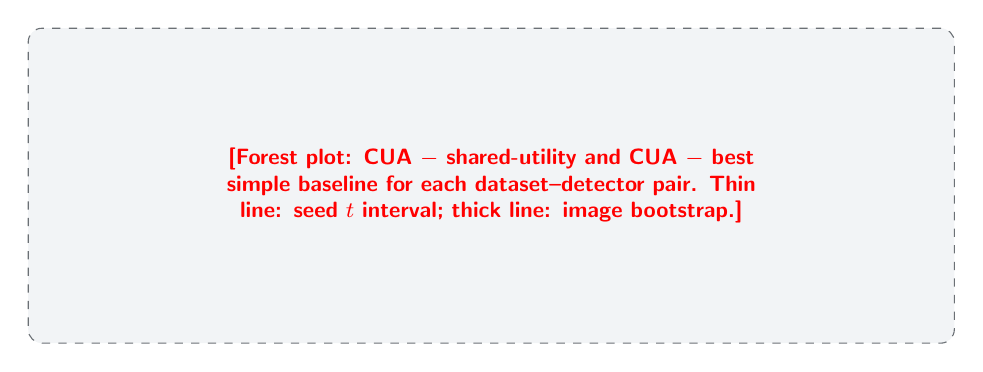
\begin{tikzpicture}
  \node[draw=cuaText, dashed, rounded corners=5pt, fill=cuaGrey!45, minimum width=0.97\columnwidth, minimum height=4cm, text width=0.8\columnwidth, align=center, font=\sffamily\footnotesize] {\todo{Forest plot: CUA $-$ shared-utility and CUA $-$ best simple baseline for each dataset--detector pair. Thin line: seed $t$ interval; thick line: image bootstrap.}};
\end{tikzpicture}
\caption{\todo{Caption written with the results.}}
\label{fig:forest}
\end{figure}

\begin{figure}[t]
\centering
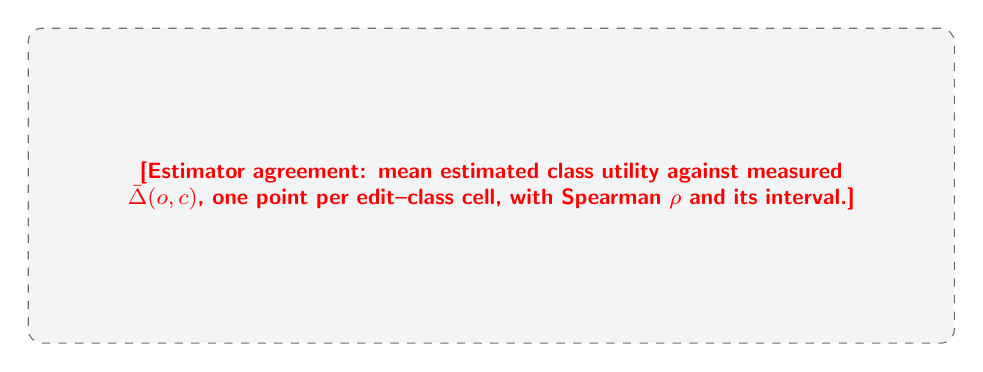
\begin{tikzpicture}
  \node[draw=cuaText, dashed, rounded corners=5pt, fill=cuaGrey!45, minimum width=0.97\columnwidth, minimum height=4cm, text width=0.8\columnwidth, align=center, font=\sffamily\footnotesize] {\todo{Estimator agreement: mean estimated class utility against measured $\bar\Delta(o,c)$, one point per edit--class cell, with Spearman $\rho$ and its interval.}};
\end{tikzpicture}
\caption{\todo{Caption written with the results.}}
\label{fig:agreement}
\end{figure}

\begin{table}[t]
\caption{Ablations of CUA on Validation (Faster R-CNN, Three Seeds)}
\label{tab:ablations}
\centering
\footnotesize
\todo{No harm block; no identity candidate; inverse-AP class weights; on RDD2022 and dacl10k.}
\end{table}

\section{Discussion and Limitations}
\label{sec:discussion}

\todo{Discussion, written with the policy comparison: when class information helps, and what it costs.}

\noindent\textbf{Limitations.} The per-class effects were measured in short continuations, and their agreement with full training was checked on one dataset and one detector only, with a wide interval. We did not run a class-targeted study that applies an edit only inside the boxes of one class, so the measured effects combine the direct effect of an edit on a class with its effect through the other objects and the background. We also did not compare CUA with a tolerance-gated controller, so the advantage of a benefit signal over a recognition signal is argued in Section~\ref{sec:related} rather than measured. Each edit has a single strength, the labels are boxes rather than masks, copy-paste augmentation is not covered, and the evaluation spans three domains. Finally, CUA is evaluated with Faster R-CNN and RetinaNet only; extending it to real-time detectors such as YOLO~\cite{bochkovskiy2020yolov4} is left to future work.


\bibliographystyle{IEEEtran}
\bibliography{references}

\end{document}
